\begin{figure*}[!ht]
\centering
  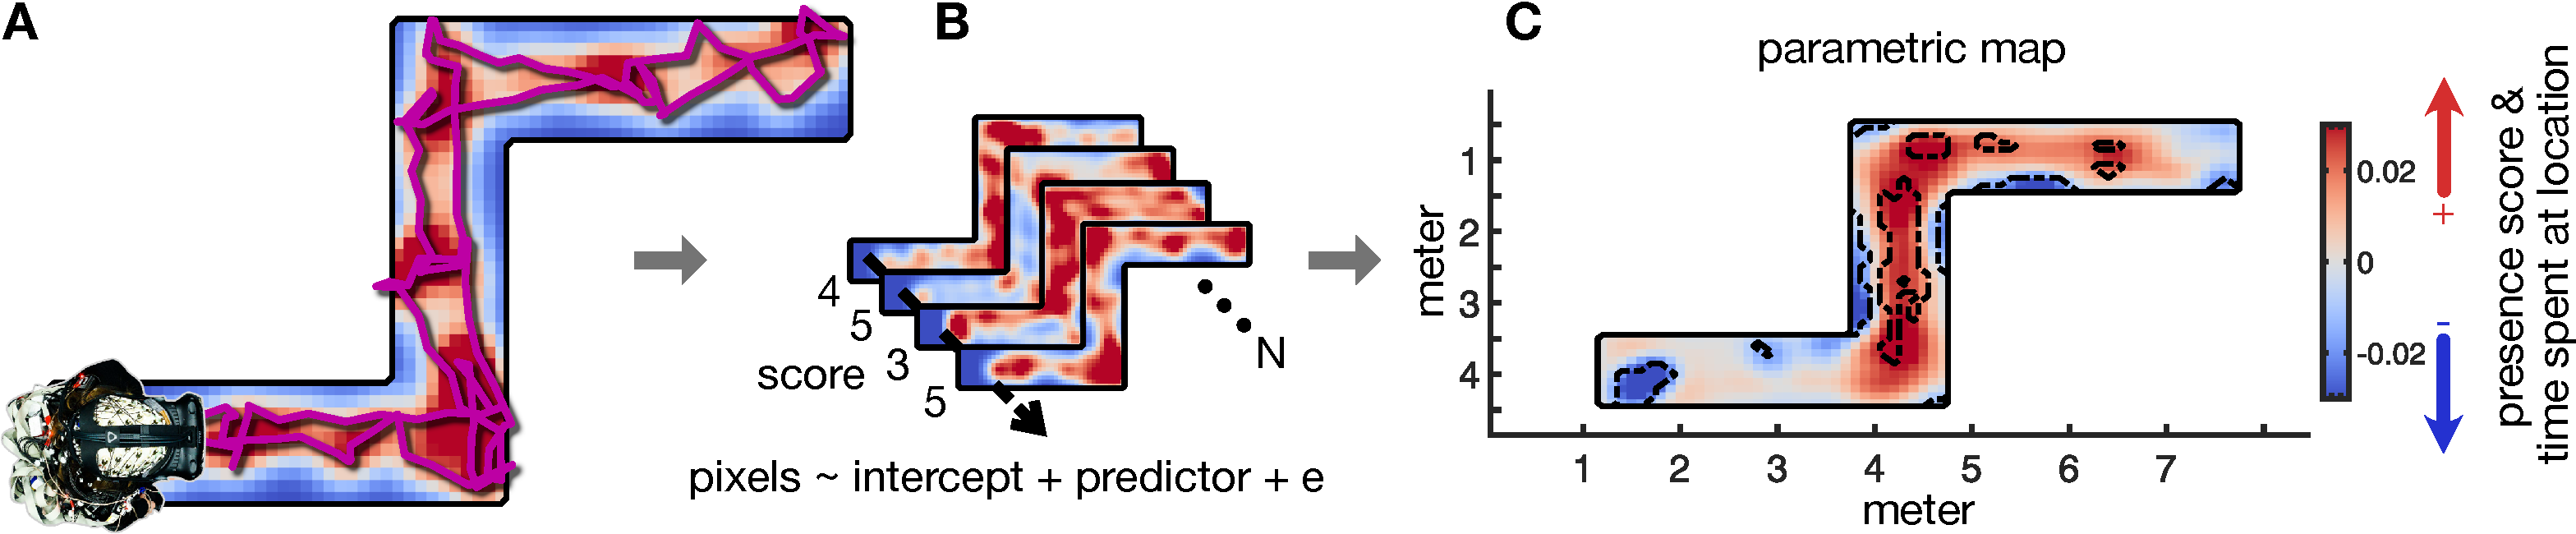
\includegraphics[width=\linewidth]{figures/fig1.pdf}
  %\vspace{-15pt}
  \caption{We propose parametric maps to guide future design decisions of room scale VR applications addressing a broader public. In our study participants explored \textit{invisible} mazes probing hidden walls for visual guidance. \textbf{A:} Motion capture of exploration paths was spatially blurred for across participants analyses of moderating variables. \textbf{B:} We administered experience presence and constructed parametric maps of where participants spent time exploring the mazes as a function of their experienced presence. \textbf{C:} Validating our proposal, we found that with increasing presence, participants were more likely to stay in the center of the paths as well as in segments critical for navigational success.}~\label{fig:methods}
\end{figure*}

% What were the previous solutions?
\section{2 Related Work}
% todo:
% - short intro to presence
In VR, illusions of various kinds (place illusion, plausibility illusion, etc.) occur at the same time for the user to feel present. Most prominently, the embodiment illusion has proven to elicit \textit{realistic} behavioral as well as physiological responses, when a strong emotional stimulus such as virtual hurting of an embodied rubber hand is provided. Such illusions enrich and/or modify participants subjective experience in VR \cite{Gonzalez-Franco2017}. Depending on the effectiveness of the employed illusions and whether multiple illusions work in congruence, participants experience feeling present in VR. 

\subsection{\textit{Natural} behavior as a precursor of presence experience}
Today, humans are still developing predominantly interacting with a physical reality. Growing up, the human brain develops its models about the worlds behavior to make useful predictions about future states \cite{} %clark. % this can now be improved a lot 

Therefore, successful immersion into virtual worlds relies on matching expectations that were substantiated in the non-virtual physical reality. Assuming that to experience presence in virtual environments equals treating what you perceive as a part of the reality you are currently in, many researchers have argued for an increase in ecological validity through VR experimentation across the cognitive sciences \cite{Bohil2011, Parsons2015, Parsons2017}. The assumption hence is that participants under the influence of successful VR illusions experience presence and therefore behave \textit{realistically} or with higher ecological validity.

% - cite studies with interesting findings but not spatially resolved, i.e. grand-averaged
%Problems of prior research in terms of the resolution of behavioral parameters investigate with respect to proteus effect or other. collapsing behavioral parameters to singular events
\subsection{Presence and behavior} % todo: redo heading
However, fewer studies have investigated the impact of the effectiveness of VR illusions on rich behavioral, psychometric and bio-physiological parameters. Here, the bulk of the literature focuses on (A) emotionally charged stimulus material or (B) embodiment illusions. Considering (A), \cite{Diemer2015} provide a thorough overview of the intricate interplay between presence and reactions to emotionally charged stimulation in VR. The authors observed a consistently reported link between presence and the emotional experience in VR. They argue, that by varying degrees of arousal, presence impacts psychological as well as physiological responses. Considering (B), we highlight one relevant aspect from the rich literature on the effects of full-body embodiment into avatars \cite{Maister2015}. The proteus effect characterizes behavioral perturbations depending on avatar body attributes. Yee et al. showed that participants being immersed into an 'attractive' avatar moved closer into the interpersonal space of another person \cite{Yee2007}. Further, Banakou et al. demonstrated that within participants, the sizes of objects were overestimated while embodied into a child body compared to a non-embodied baseline \cite{Banakou2013}. These examples illustrate that the level of experienced presence directly impacts the action-perception cycle.

One of the key VR illusions contributing to the subjective construct of presence is the place illusion which can be defined as the perception of oneself being present in a virtual place where one can act, react, and impact the surroundings \cite{Slater2009}. Therefore, self-location, sense of agency, and the spatial awareness of the surroundings are strongly impacted by the place illusion and modify behavior \cite{Kilteni2012}. When one perceives oneself as in control of their own actions and observe action consequences in their virtual surroundings, spatial exploration behavior becomes a part of a learning process to adapt motor behavior to the surroundings as opposed to a random chain of actions executed by the user to explore, for instance, only the VR technology itself \cite{Tan2011}.

% - what is the benefit of spatial resolution?
% maybe explain background of spm in cognitive neuroscience?
% find examples of mocap analysis collapsing data to the mean

% Summary motivating our work: 
% - 


%%%%% writing resources
%The framework is derived from the neuroscientific methodology of parametric brain imaging, see for example \cite{Friston1994, Pernet2011}.
%mental representation of the surroundings and respectively the motor behavior.
%Novel immersive paradigms in the behavioral cognitive sciences as well as neurosciences subject participants to controlled, yet stimulus rich experiences in head-mounted VR. 
%Therefore, to be able to employ VR and claim ecological validity the level of presence must be accounted for. 